\documentclass[margin=1mm]{standalone}
\usepackage[utf8]{inputenc}
\usepackage{amsmath}
\usepackage{amsfonts}
\usepackage{amssymb}
\usepackage{tikz}
\usetikzlibrary{calc,arrows,positioning,shapes,shapes.gates.logic.US,trees, backgrounds}

\begin{document}
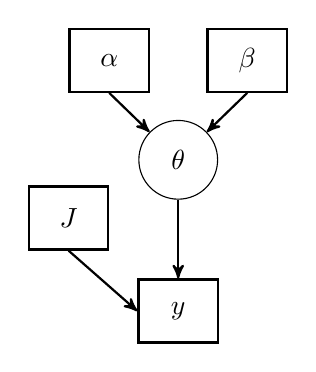
\begin{tikzpicture}[auto,scale=3,
	latent/.style={circle,draw,thick,text badly centered, inner sep=2pt,minimum size=20mm, text width=4.5em, fill=white},
	error/.style={circle,draw,text badly centered, inner sep=2pt,minimum size=10mm},
	manifest/.style={text centered, rectangle,draw,thick,inner sep=3pt,minimum height=8mm, minimum width=8mm, text width= 8 mm},
	manifestRot/.style={text centered, rectangle, draw, thick,inner sep=3pt, minimum width=7mm, text width= 7mm, minimum height=15},
	manifestfront/.style={rectangle,draw,thick,inner sep=0pt,minimum size=12mm, fill=white},
	ghost/.style={rectangle, inner sep=0pt,text centered,    minimum height=0mm, minimum width=5mm, text width= 5 mm},
	lcorr/.style={<->,>=stealth', bend right=40},
	rcorr/.style={<->,>=stealth', bend left=40},
	fcorr/.style={<->,>=stealth', bend left=40},
	ofcorr/.style={<->,>=stealth', bend right=60},
	ofcorr2/.style={<->,>=stealth', bend left=60},
	intercept/.style={regular polygon,
        regular polygon sides=3,draw,thick,inner sep=0pt,minimum size=10mm},
	mean/.style={regular polygon,regular polygon sides=3,draw,thick,inner sep=0pt,minimum size=10mm},
	paths/.style={->, thick, >=stealth'},
	variance/.style={<->, thick, >=stealth', bend left=270, looseness=2},
	varianceTop/.style={<->, thick, >=stealth', bend right=270, looseness=2},
	unique/.style={<->, thick, >=stealth', loop below=270, looseness=8},
	factvar/.style={<->, thick, >=stealth', loop right=270, looseness=8}
	] % End Creating Path Model Pieces
\tikzset{mystyle/.style={->,double=black}}


\node [error] at (0,0) (t) {$\theta$};
\node [manifest] [below = 1cm of t] (y) {$y$};
\node [ghost] [above = 0.75cm of t]  (g) {};
\node [manifest] [left = 0.1cm of g] (a) {$\alpha$};
\node [manifest] [right = 0.1cm of g] (b) {$\beta$};
\node [manifest] [above left = 0.5cm of y] (j) {$J$};

\draw[paths] (t) -- (y);
\draw[paths] (j.south) -- (y.west);
\draw[paths] (a.south) -- (t);
\draw[paths] (b.south) -- (t);

\end{tikzpicture}
\end{document}